\documentclass{subfiles}


\begin{document}

\section{Background Information}
		\par {\color{red} *** Neill: the following paragraphs were moved here from the Background Chapter 1.2}
		
		\par The most common approach of interpreting the FW LiDAR is the Gaussian decomposition of the waveforms and extraction of peak points ~\cite{Wanger2006}. Neunschwander et al used this approach for Landcover classification while Reitberger et al applied it for distinguishing deciduous trees from coniferous trees ~\cite{Neuenschwander2009}~\cite{Reitberger2008}. Chauve et al further proposed an approach of improving the Gaussian model in order to increase the density of the points extracted from the data and consequently improve point based classifications of FW LiDAR data ~\cite{Chauve2007}. 
		
		\par While echo decomposition identifies significant features as points, the FW LiDAR data also contains information in single shots that may be below the significance threshold. The waveform samples data can be accumulated from multiple shots into {\color{blue} into a voxel array, building up a 3D density volume. The correlation between multiple pulses into a voxel representation produces a more accurate representation, which confers greater noise resistance and it further opens up possibilities of vertical interpretation of the data.} Voxelisation {\color{blue} of FW LiDAR data} was firstly introduced by Persson et al, who used it to visualise the waveforms using different transparencies \cite{Persson2005} and it seems to be the future of FW LiDAR data with the literature moving toward that direction. In 2016, Cao et al used it for tree species identification \cite{Cao2016} and Sunmall et al characterised forest canopy from a voxelised vertical profile \cite{Sumnall2016}. This innovative approach is an integral part of this thesis and it is used for both visualisations and classifications \cite{Miltiadou2014}\cite{Miltiadou2015}. 
		\par {\color{red} *** end of moved paragraphs *** }
		
		

	
\section{Explanation of Voxelisation}


\par The FW LiDAR data are voxelised by inserting the wave samples into a 3D regular grid and constructing a 3D discrete density volume. According to Person et al, each wave sample is associated with the 3D cell, named voxel, that it lies inside. If multiple samples lie inside a voxel then the sample with the highest intensity is chosen ~\cite{Persson2005}. In order to reduce noise, there are two differences between this approach and the way FW LiDAR data are voxelised in DASOS. 

\par At first a threshold is used to remove low level noise, because when the width of a recorded waveform is longer that the distance between the first hit point and the ground, the system captures low signals, which are pure noise. For that reason, the samples with intensity lower than a user-defined noise level/threshold are discarded. 

\par Then each wave sample is associated with the voxel that it lies inside and the second difference is how DASOS overcomes the uneven number of samples per voxels. The intensity of each sample is the laser intensity returned during the corresponding time interval. For example, if 5 samples are inside a voxel and the waveform is digitised at 2ns, then the laser intensity associated with that voxel corresponds to 10ns waveform width. For comparison purposes, it's essential to keep the waveform width consistent across the voxels. For overcoming this issue in DASOS, the average intensity of the samples that lie inside each voxel is taken, instead of choosing the one with the highest intensity ~\cite{Persson2005}. This way the likelihood of the 3D volume to be affected by outliers and high noise is reduced. The following equation shows how the intensity value of a voxel is calculated:
 
	\begin{eqnarray}
	I_{v} = \dfrac{\sum_{i=1}^{n}I_{i}}{n}
	\end{eqnarray} 
	where 		$I_{v}$ is the accumulated intensity of voxel $v$. 
	$n$ is number of samples associated with that voxel, 
	$I_{i}$ is the intensity of the sample i, 

To sum up, during voxelisation the area of interest is divided into voxels. The samples of the FW LiDAR data are inserted inside this 3D discrete density volume and normalised such that equally sized waveform width is saved inside each voxel. The result is a 3D discrete density volume of the scanned area. Figure \ref{fig:Voxelisation} depicts this process in 2D.


\begin{figure} [h!]

\begin{subfigure}[t]{.31\textwidth}
	\centering
	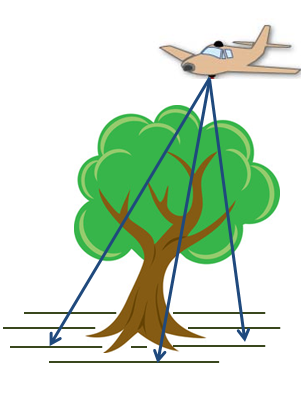
\includegraphics[width=.9\textwidth]{img/VoxelisationA}
	\caption{The sensor from the plane emits multiple pulses and collects information from the return.}
	\label{fig:VoxelisationA_scan}
\end{subfigure} \hfill
\begin{subfigure}[t]{.31\textwidth}
	\centering
	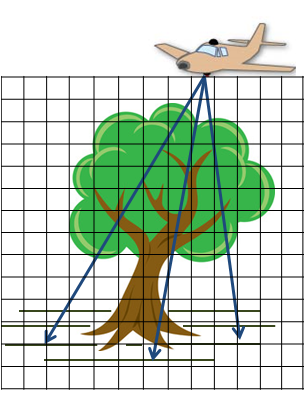
\includegraphics[width=.9\textwidth]{img/VoxelisationB}
	\caption{The area of interest is divided into equally space cubes, named voxels, generating this way a discrete volume.} 
	\label{fig:VoxelisationB_grid}
\end{subfigure} \hfill
\begin{subfigure}[t]{.31\textwidth}
	\centering
	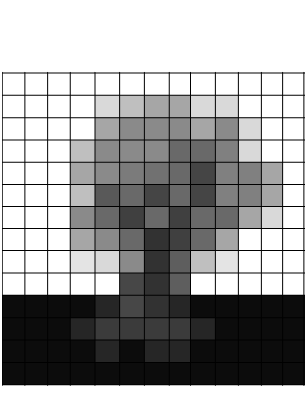
\includegraphics[width=.9\textwidth]{img/VoxelisationC}
	\caption{The accumulated intensities of wave samples into the volume builds up the voxelised representation of the scanned area.} 
	\label{fig:VoxelisationC_voxelised}
\end{subfigure}
\caption[Voxelisation of FW LiDAR data]{The above images depict the voxalisation process of the FW LiDAR data in 2D. Please note that the voxelisation output in Figure \ref{fig:VoxelisationC_voxelised} shows how ideally the result would look like. But in reality, trees may be disconnected from the ground due to missing information about the trunk.}
\label{fig:Voxelisation}
\end{figure}


\section{Implicit Object}

\par Once the 3D discrete density volume is generated, an implicit object is defined to represent the scanned area. Implicit objects were introduced by Blinn in 1982 \cite{Blinn1982} and enable the definition of complex objects without saving a large amount of triangles. Each one is defined by a function $ \mathit{f(X)} $ and the iso-surface value $\alpha$. The iso-surface value defines the boundaries of the object; for an object $ [f(x),a]$ every n-dimensional point $ \mathit{X} $  that lies on the surface of the object satisfies the condition $ \mathit{f(X)=\alpha }  $. To be more specific, all the following rules apply according to Pasko et al \cite{Pasko1994}: 
\begin{itemize}
	\item $	\mathrm{f(X) = \alpha }$ , when $X$ lies on the surface of the implicit object
	\item $	\mathrm{f(X) > \alpha }$ , when $X$ lies inside the implicit object and
	\item $	\mathrm{f(X) < \alpha }$ , when $X$ lies outside the implicit object	 
\end{itemize}


\par Regarding the implicit representation of the 3D voxelised FW LiDAR, X is a three dimensional point $\mathit{(x, y, z) }$ representing the longitude, latitude and height respectively and ${f(X)}$ is a function that takes  $\mathit{X}$ as input and returns the accumulated intensity value of the voxel that  $\mathit{X}$ lies inside. Also, the iso-surface value $\mathit{\alpha }$ is a user defined parameter and it is noise dependant (Please look at figure *** to understand how the iso-surface value affects the implicit representation of voxelised FW LiDAR data). 


\section{Conclusions}
This thesis strongly supports voxelisation of FW LiDAR data. Voxelisation preserves information beyond the significant threshold of point extraction algorithms. It further accumulates intensity values from multiple shots and stores them into a 3D regular grid, resolving this way the sinusoidal footprints pattern of the Leica system; all the voxel values are normalised and contain an intensity value that corresponds to equal waveform width. Voxelisation is further supported by the recent literature \cite{Cao2016} \cite{Sumnall2016}. 

In a few words, the FW LiDAR data are voxelised by inserting the wave samples into a 3D discrete density volume. Then an implicit representation of that volume is defined by the function $f(X)$ and the iso-surface value $\alpha$. The function $f(X)$ takes as input a point $X$ and returns the associated intensity of the voxel that $X$ lies inside. If the returned intensity is greater than the value $\alpha$ then $X$ lies inside the implicit object, if it is is equal to $\alpha$ then it is on the boundary otherwise it lies outside. 



\end{document}